%!TEX root = ../template.tex
%%%%%%%%%%%%%%%%%%%%%%%%%%%%%%%%%%%%%%%%%%%%%%%%%%%%%%%%%%%%%%%%%%%%
%% 4-Work_Done.tex
%% NOVA thesis document file
%%
%% Chapter with the template manual
%%%%%%%%%%%%%%%%%%%%%%%%%%%%%%%%%%%%%%%%%%%%%%%%%%%%%%%%%%%%%%%%%%%%

\typeout{NT FILE 6-Generalized_Development.tex}%

\chapter{Generalized Development}
\label{cha:Generalized Development}

\glsresetall

\section{Introduction} \label{sec.6:Introduction}
This section will focus on the generation of the architecture so that the encirclement may use other shapes other then the two-sphere, this generation as will be shown allows for some useful use cases associated with the restricted aerial space use case. 
As in previous chapters first the new architecture will be shown and explained being the base the Decentralized version demonstrated in Chapter~\ref{cha:Decentralized Development}.

\section{Agent distributions}

As previously mentioned this version is not only useful for the two sphere but also other shapes, in Figure~\ref{fig.6:llyod_dijkstra_algorithm_distribution} is is possible to see the distribution of 1001 agents using a new method also based on the voronoi method but in this case using the disktra method in order to obtain the new centroid center \gls{voronoi_centroid}. In Figure~\ref{fig.6:llyod_dijkstra_algorithm_distribution_stl} it is possible to see the distribution of 8 agents in two meshes obtain from stl files of the dataset thingi10k\cite{zhouThingi10KDataset100002016}, a data set with 10 thousand stl's from thingiverse \cite{thingiverse_website}

\begin{figure}[htbp]
    \centering
    \subfloat[Normal]{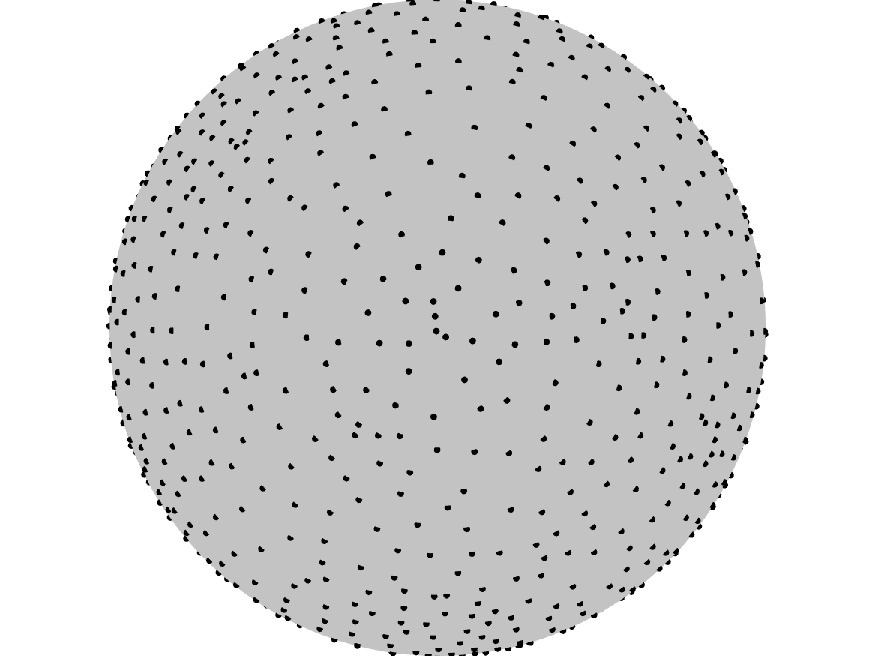
\includegraphics[width=3cm]{5-Figures/Chapter3/Lloyd_disktra/Voronoi_dijkstra_normal.pdf}}\hfil
    \subfloat[Top]{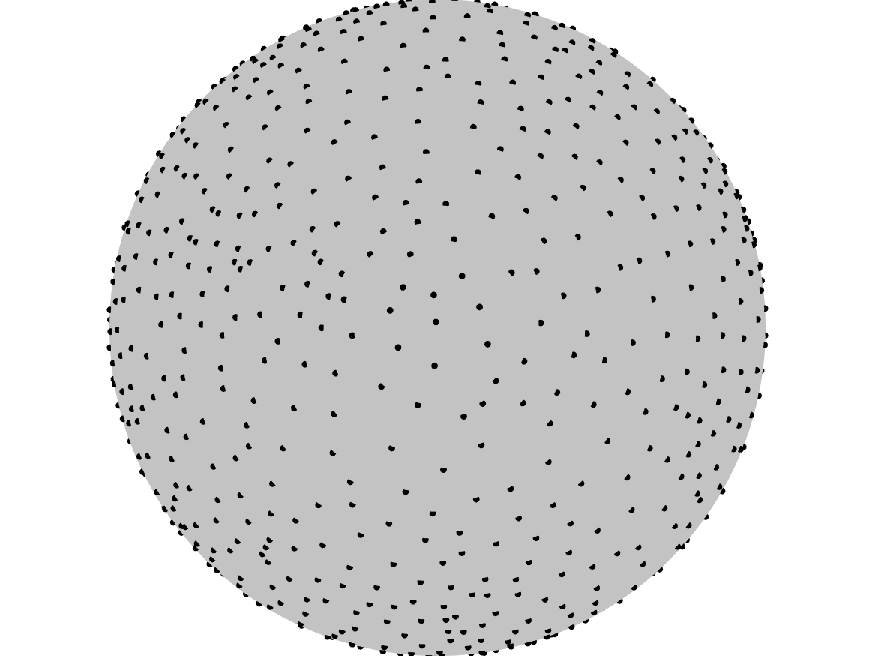
\includegraphics[width=3cm]{5-Figures/Chapter3/Lloyd_disktra/Voronoi_dijkstra_top.pdf}}\hfil
    \subfloat[Side]{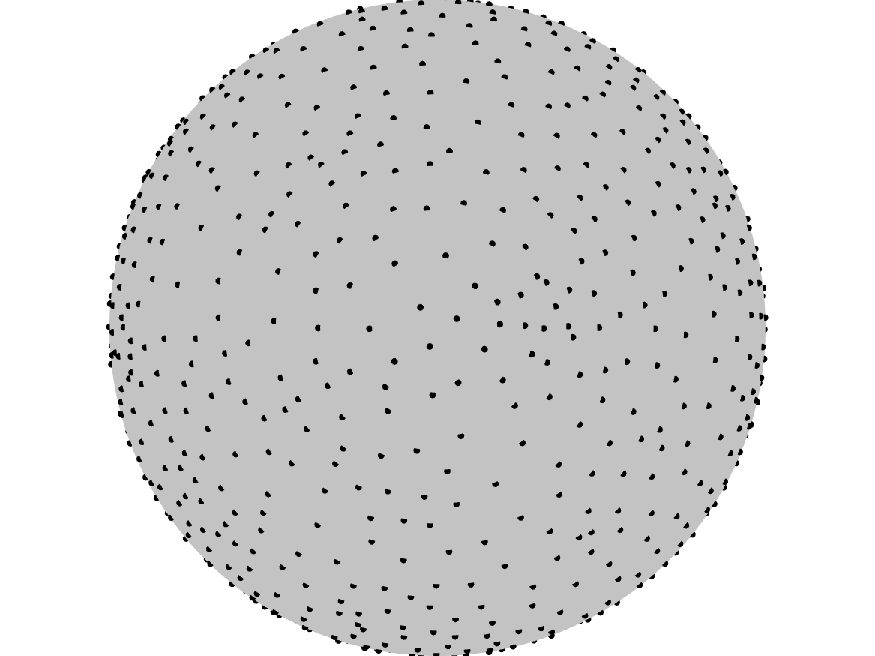
\includegraphics[width=3cm]{5-Figures/Chapter3/Lloyd_disktra/Voronoi_dijkstra_side.pdf}}
    \caption{Lloyd's algorithm (dijkstra) distribution. (1001 points)}
    \label{fig.6:llyod_dijkstra_algorithm_distribution}
\end{figure}

The spacing between agents is not desirable but this is due to the graphical limitation of the computer used for simulation since the mesh verticies define the positions each site can be located (this is implementation dependent) and for the use of 1001 sites a mesh of 10000 points was used, this points where placed using the fibonacci lattice method to ensure the mesh formation was as even as possible, ensuring a better site distribution on the mesh. The dijkstra method used in this implementation not only can only place sites on the location of vertices of the underlying mesh but also requires for the underlying mesh to be well defined (evenly spread forming the desired shape).

\begin{figure}[htbp]
    \centering
    \subfloat[Bust]{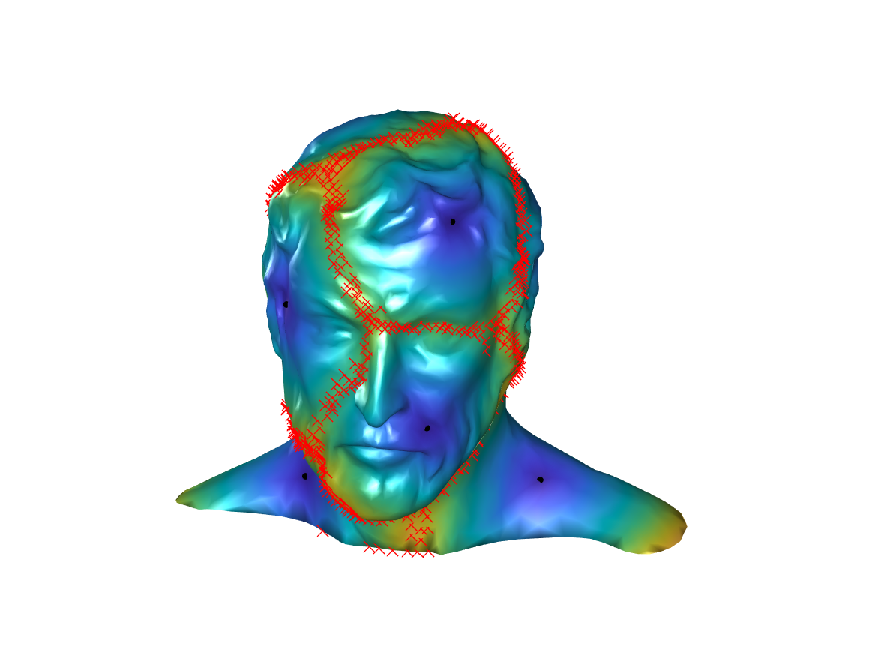
\includegraphics[width=6cm]{5-Figures/Chapter6/Voronoi_dijkstra_bust.pdf}}\hfil
    \subfloat[Frog]{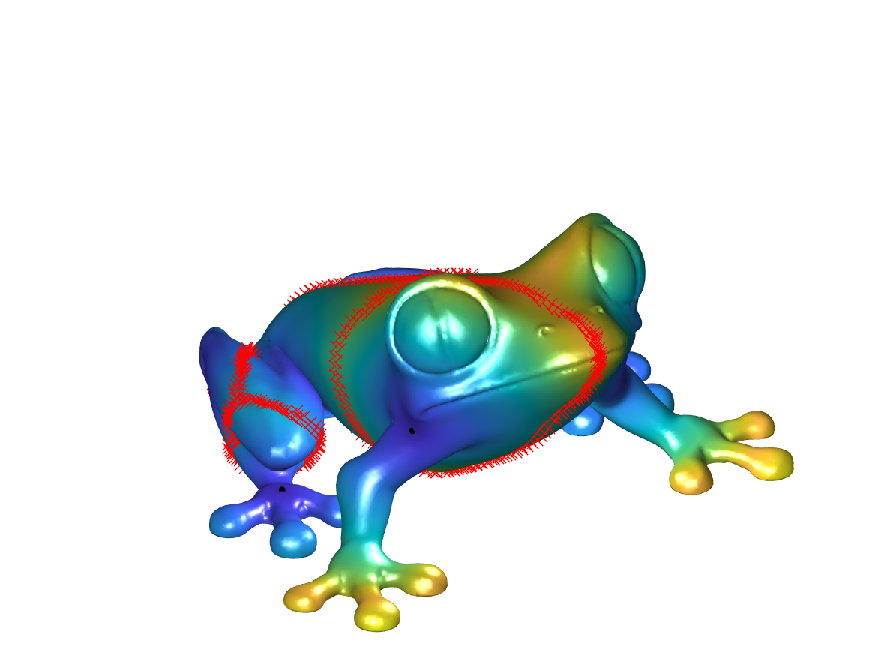
\includegraphics[width=6cm]{5-Figures/Chapter6/Voronoi_dijkstra_frog.pdf}}
    \caption{Lloyd's algorithm (dijkstra) distribution. (8 points)}
    \label{fig.6:llyod_dijkstra_algorithm_distribution_stl}
\end{figure}

In the Figure~\ref{fig.6:llyod_dijkstra_algorithm_distribution_stl} it is possible to visualize the sites as black dots the distance from said points via the surface gradient being colder colors closer to a site and warmer color further away and finally any point defined as a Voronoi edge marked with a red cross, with these two examples it is possible to see that this distribution is capable of separating points on any well defined mesh. 

\section{Control architecture}

As has been previously mentioned in the introduction the architecture of the control system has been simplified since the geometric controller and the radial controller are no longer used, assuming that the agents/drones are initialized in the mesh as sites or the mesh is initialized in a way that encompasses all agents, the Mellinger controller has as a direct reference the final desired position, in this case the updated sites of the Voronoi. In Figure~\ref{fig.6:generalized_controller_architecture} it is possible to see the new architecture of the system with the added mesh controller responsible for given the position of the target modify the position and shape of the mesh.

\begin{figure}[htbp]
  \centering
  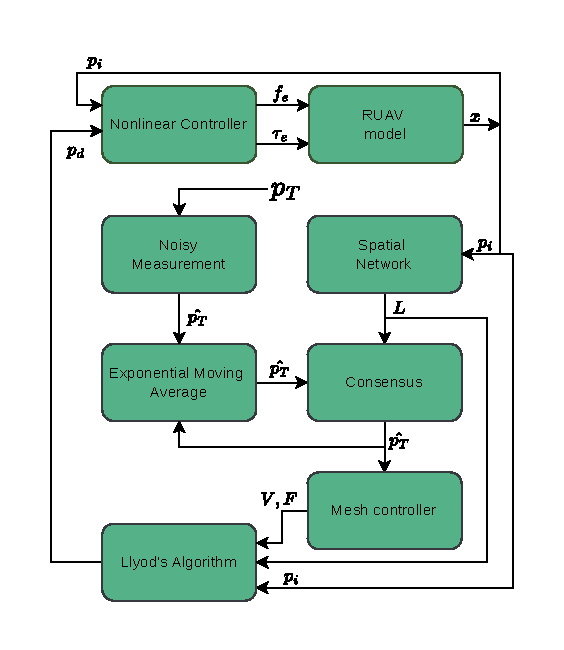
\includegraphics[width=0.85\textwidth]{5-Figures/Chapter6/controller_architecture/genrelized_complete_controller_architecture.drawio.pdf}
  \caption{Generalized controller architecture}
  \label{fig.6:generalized_controller_architecture}
\end{figure}

\subsection{Mesh Controller}

The mesh controller is responsible for dynamically modifying the shape of the mesh (i.e., the position of its vertices) according to the relative position of a target with respect to a restricted airspace. The objective is to ensure that a swarm of drones, located at the boundary of this region, can physically block or contain the target while avoiding collisions.

When the target is outside the restricted airspace, the drones form a planar circular barrier. As the target approaches and reaches the boundary, the mesh deforms continuously by pushing the center of the circle inward, preventing penetration while maintaining a safe distance. If the target moves further inside—specifically more than one radius length—the mesh transitions into a closed spherical configuration, fully enclosing the target.

In Figure~\ref{fig:mesh_controller_demonstration}, a mesh composed of $P = 1001$ vertices is shown, with a target (red point) located at positions corresponding to the three stages. The radius of the circle and sphere is $R = 5$.

\begin{figure}[htbp]
    \centering
    \subfloat[outside]{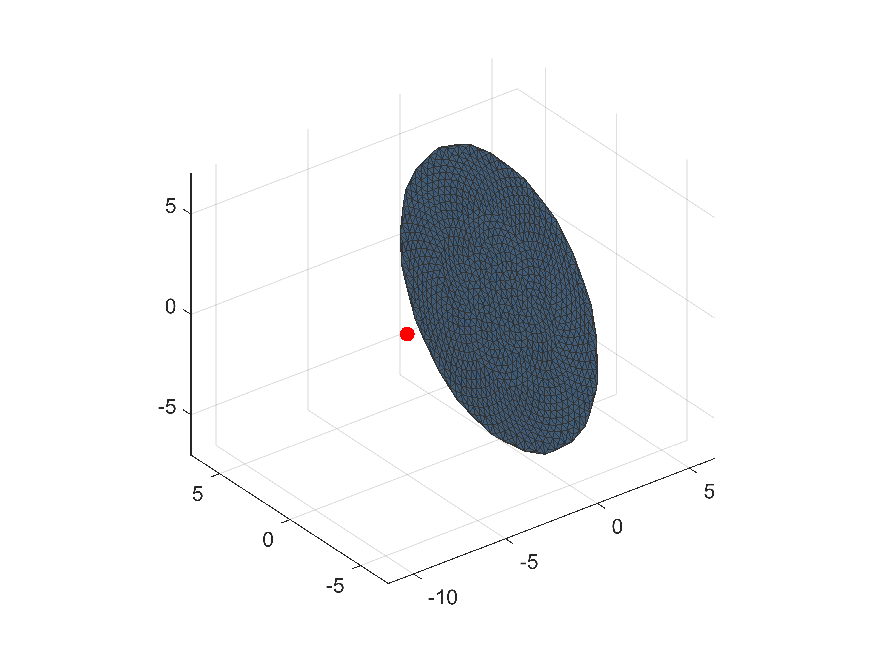
\includegraphics[width=6cm]{5-Figures/Chapter6/mesh_controller/mesh_controller_outside.pdf}}\hfil
    \subfloat[edge]{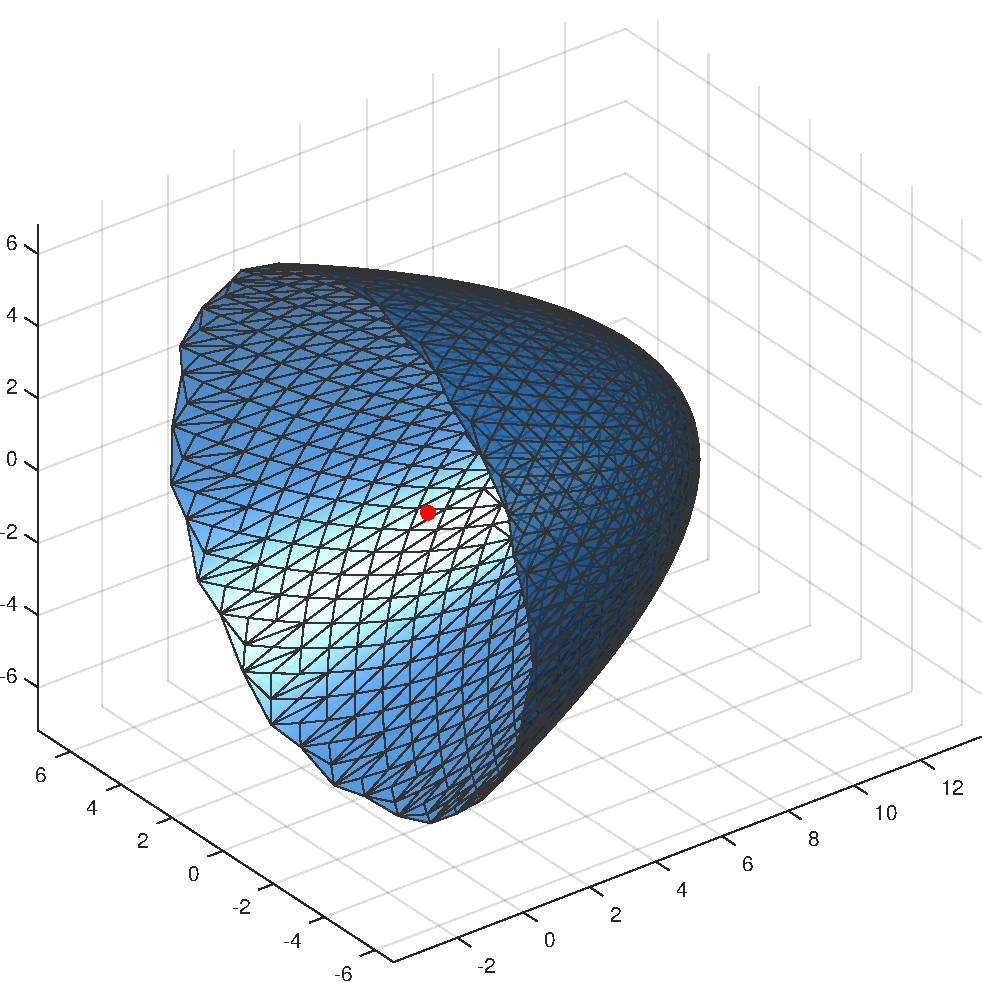
\includegraphics[width=6cm]{5-Figures/Chapter6/mesh_controller/mesh_controller_border.pdf}}\hfil
    \subfloat[inside]{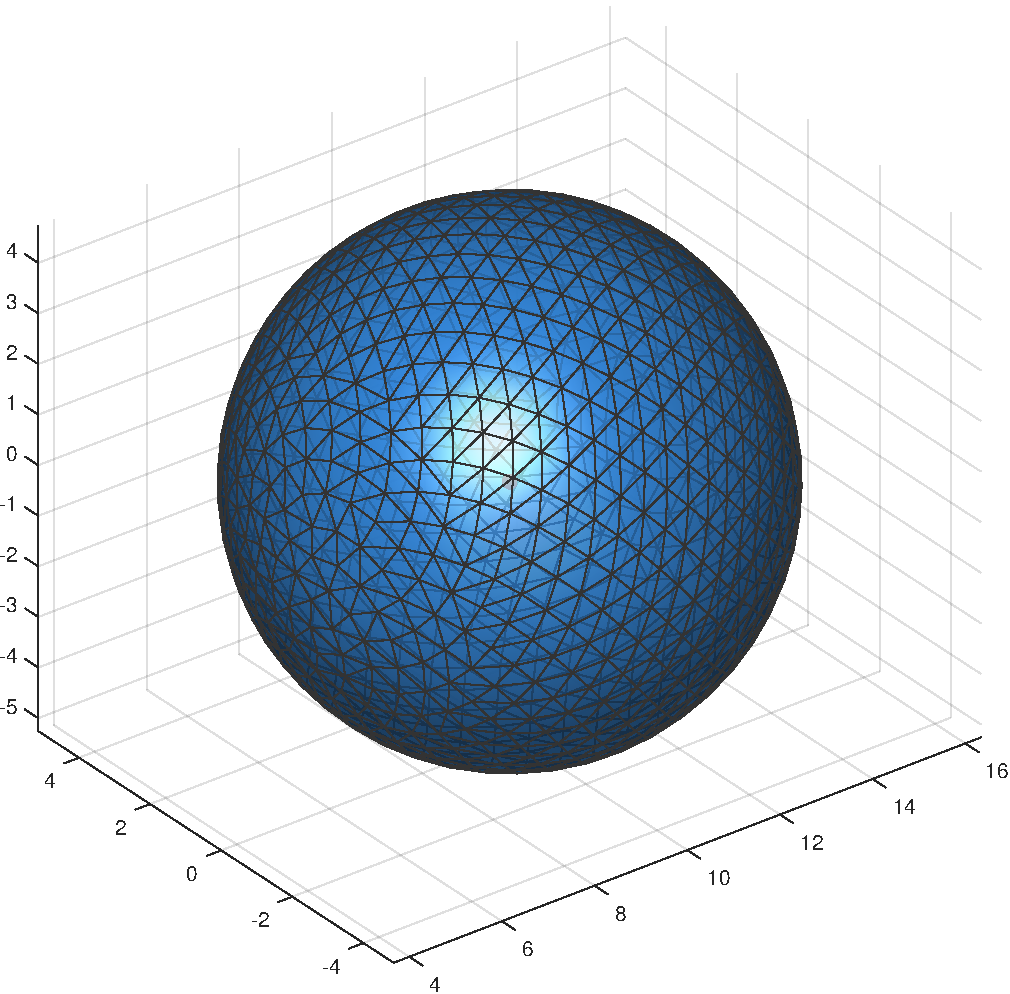
\includegraphics[width=6cm]{5-Figures/Chapter6/mesh_controller/mesh_controller_inside.pdf}}
    \caption{Mesh controller demonstration at different stages of target interaction.}
    \label{fig:mesh_controller_demonstration}
\end{figure}

The algorithm pre-computes three configurations of the mesh vertices:
\begin{itemize}
    \item A circular configuration $\mathbf{v}_{\text{circle}} \in \mathbb{R}^{P \times 3}$,
    \item A conical configuration $\mathbf{v}_{\text{cone}} \in \mathbb{R}^{P \times 3}$,
    \item A spherical configuration $\mathbf{v}_{\text{sphere}} \in \mathbb{R}^{P \times 3}$.
\end{itemize}

The final mesh is obtained through a two-stage interpolation process based on the target position $\mathbf{p} \in \mathbb{R}^3$. Let $u_1, u_2 \in [0,1]$ be interpolation parameters derived from the signed distance of the target to the surface. The intermediate mesh is defined as:

\begin{equation}
    \mathbf{v}^{(1)} = (1 - u_1)\,\mathbf{v}_{\text{circle}} + u_1\,\mathbf{v}_{\text{cone}},
\end{equation}

followed by a second interpolation:

\begin{equation}
    \mathbf{v}^{(2)} = (1 - u_2)\,\mathbf{v}^{(1)} + u_2\,\mathbf{v}_{\text{sphere}}.
\end{equation}

Thus, the final vertex positions are given by:

\begin{equation}
    \mathbf{v}_{\text{final}} = \mathbf{v}^{(2)} + \mathbf{p}_{\text{mesh}},
\end{equation}

where $\mathbf{p}_{\text{mesh}}$ is a translation term that shifts the mesh according to the target position, being $\mathbf{p}_{\text{mesh}}$ the target position if $u_2 = 1$ (full circle) or in any other case the target position is projected on the restricted airspace surface and that is the position of the $\mathbf{p}_{\text{mesh}}$.
This formulation guarantees that the mesh adapts continuously to the target position, enabling collision avoidance while maintaining containment of the target within the restricted airspace. 

The mesh connectivity (i.e., the set of edges/faces) is computed dynamically. For partially open configurations—corresponding to $u_1 \in [0,1]$ and $u_2 \in [0,0.5)$ the \(\text{MATLAB}^\text{\textregistered}\)~\cite{MATLAB:R2024a} Delaunay triangulation \cite{MATLAB_delaunay} is used, as it provides a robust connection for non-closed surfaces. Once the mesh approaches a closed shape ($u_2 \ge 0.5$), the \(\text{MATLAB}^\text{\textregistered}\)~\cite{MATLAB:R2024a} convex hull \cite{MATLAB_convhull} is computed instead, ensuring a fully enclosed 3D surface.

\section{Simulation results}

In this section, the simulation results are presented and discussed. The scenario consists of a target that moves in a circular trajectory, alternating between inside and outside the restricted airspace. A total of 12 agents are initially deployed on the mesh. The Voronoi update is the only component of the system that is not executed at every time step due to its computational cost; instead, it is performed every 100 time steps (once per second).

During the simulation, the loss of three agents mid-flight, $t = 5$ sec, due to no control input (simulating loss of power) is also introduced to demonstrate the resilience of the system. As in the previous version, all agents operate in a fully decentralized manner and communicate through a spatial network. This allows them to collaboratively estimate the target's position, as well as exchange information about their own positions with neighboring agents in order to update the Voronoi diagram. In Figure~\ref{fig.6:simulation_results} it is possible to see the how the mesh and agents move through space and time.

\begin{figure}[htbp]
\centering
\begin{minipage}{0.12\textwidth}
t = 0.5:
\end{minipage}%
\begin{minipage}{0.85\textwidth}
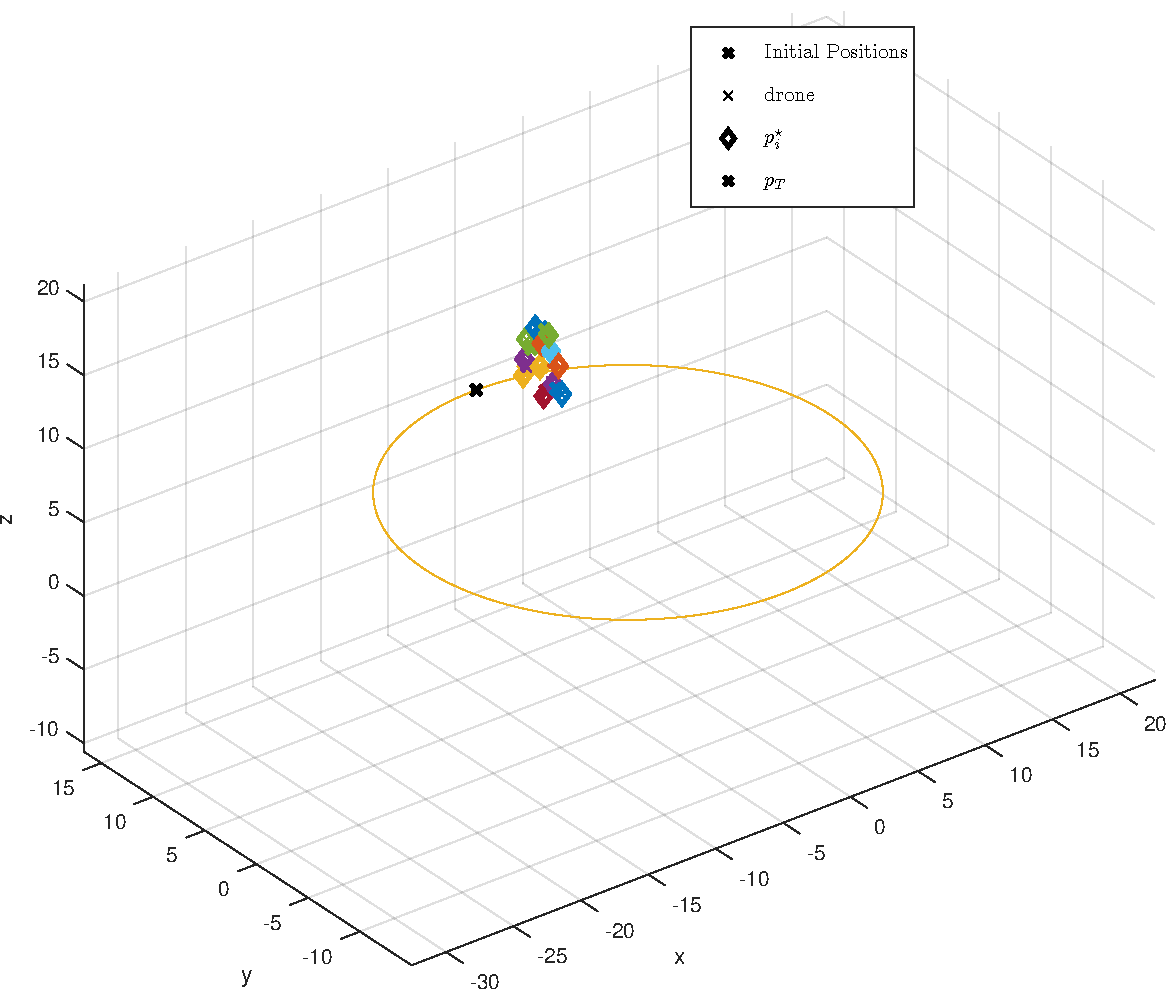
\includegraphics[width=6cm]{5-Figures/Chapter6/Simulation/decentralized_dijktra_t_0.5.pdf}\hfil   
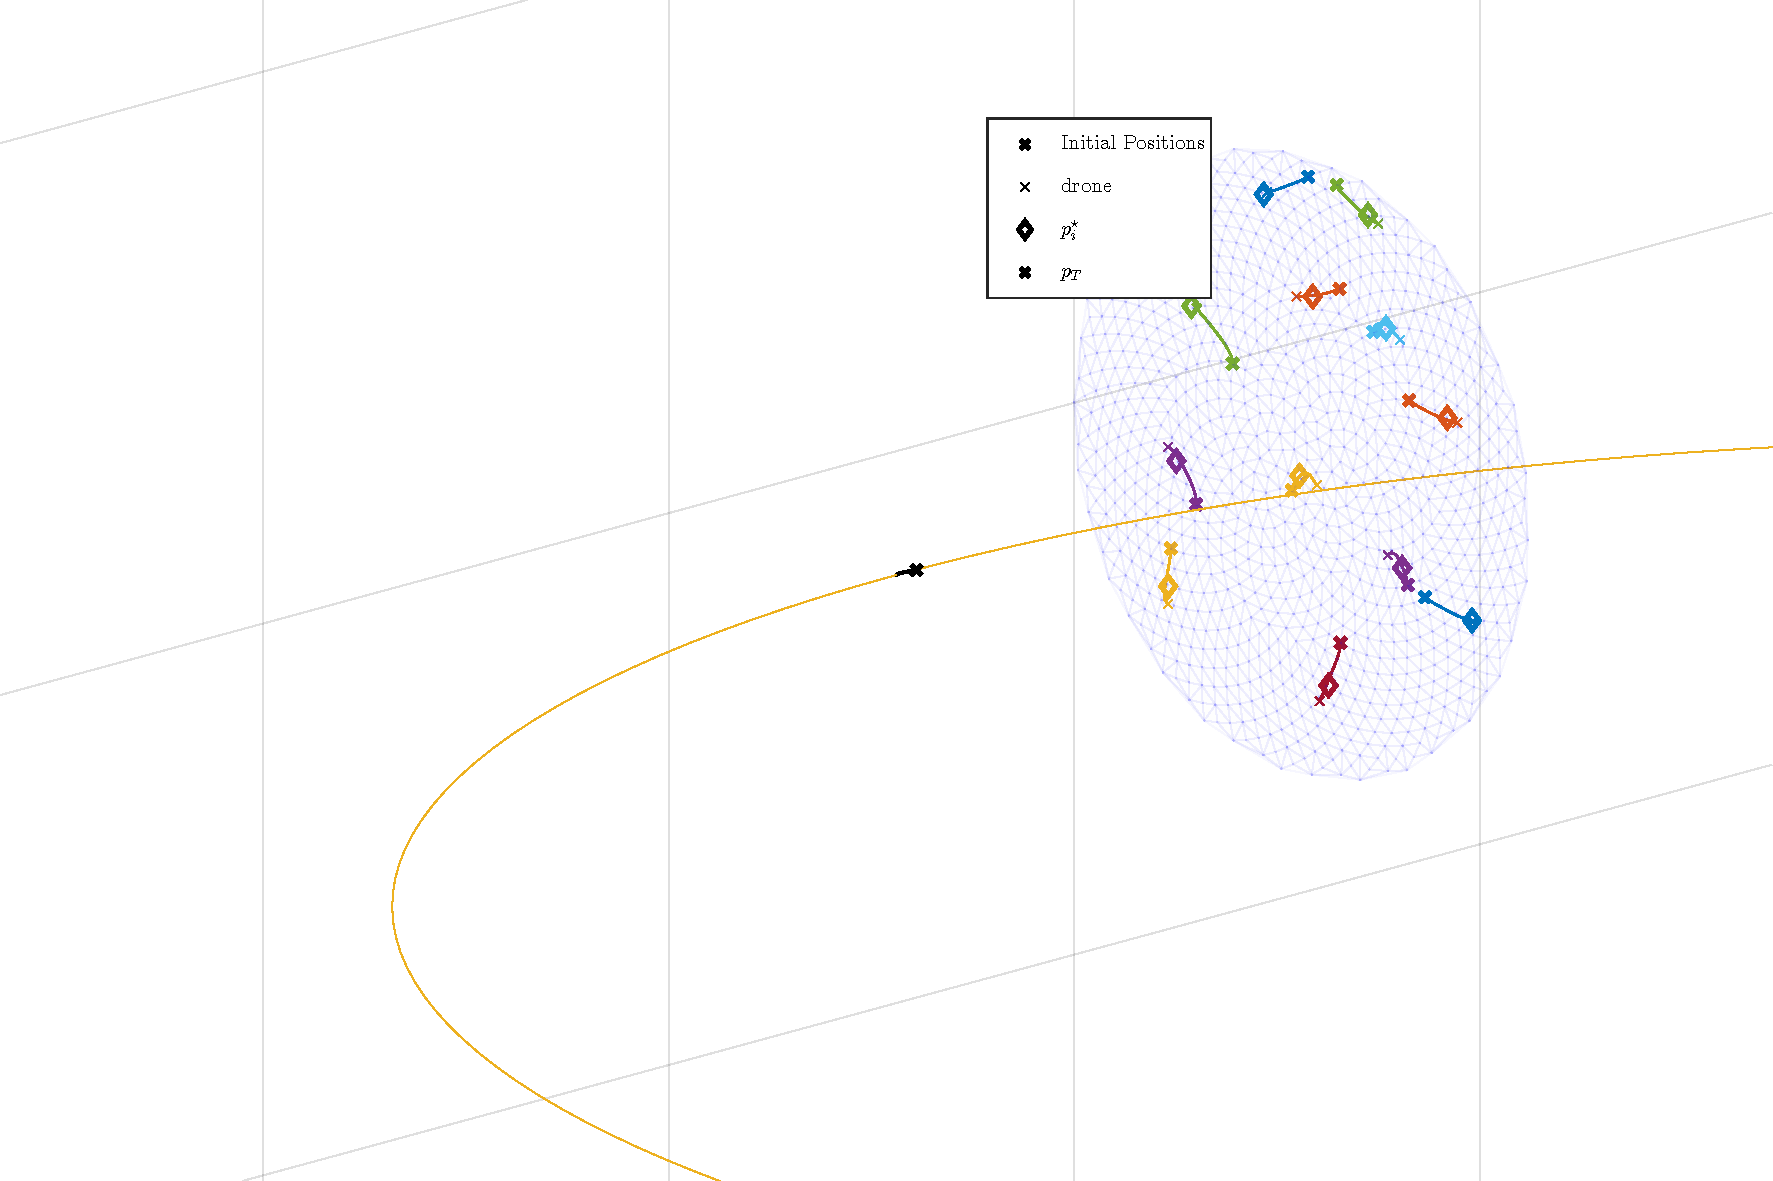
\includegraphics[width=6cm]{5-Figures/Chapter6/Simulation/decentralized_dijktra_t_0.5_close.pdf}
\end{minipage}

\vspace{0.3cm}

\begin{minipage}{0.12\textwidth}
t = 3:
\end{minipage}%
\begin{minipage}{0.85\textwidth}
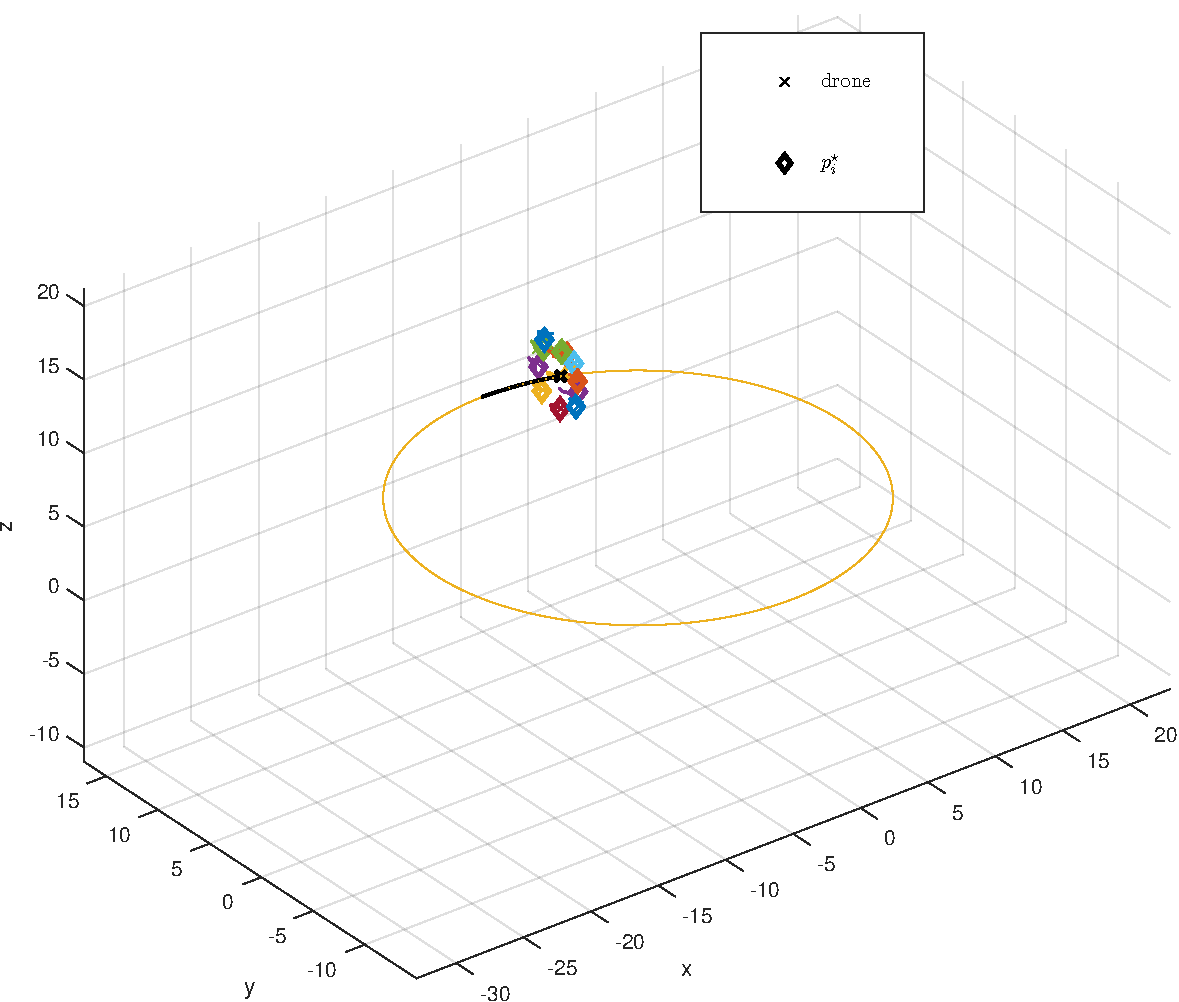
\includegraphics[width=6cm]{5-Figures/Chapter6/Simulation/decentralized_dijktra_t_3.pdf}\hfil   
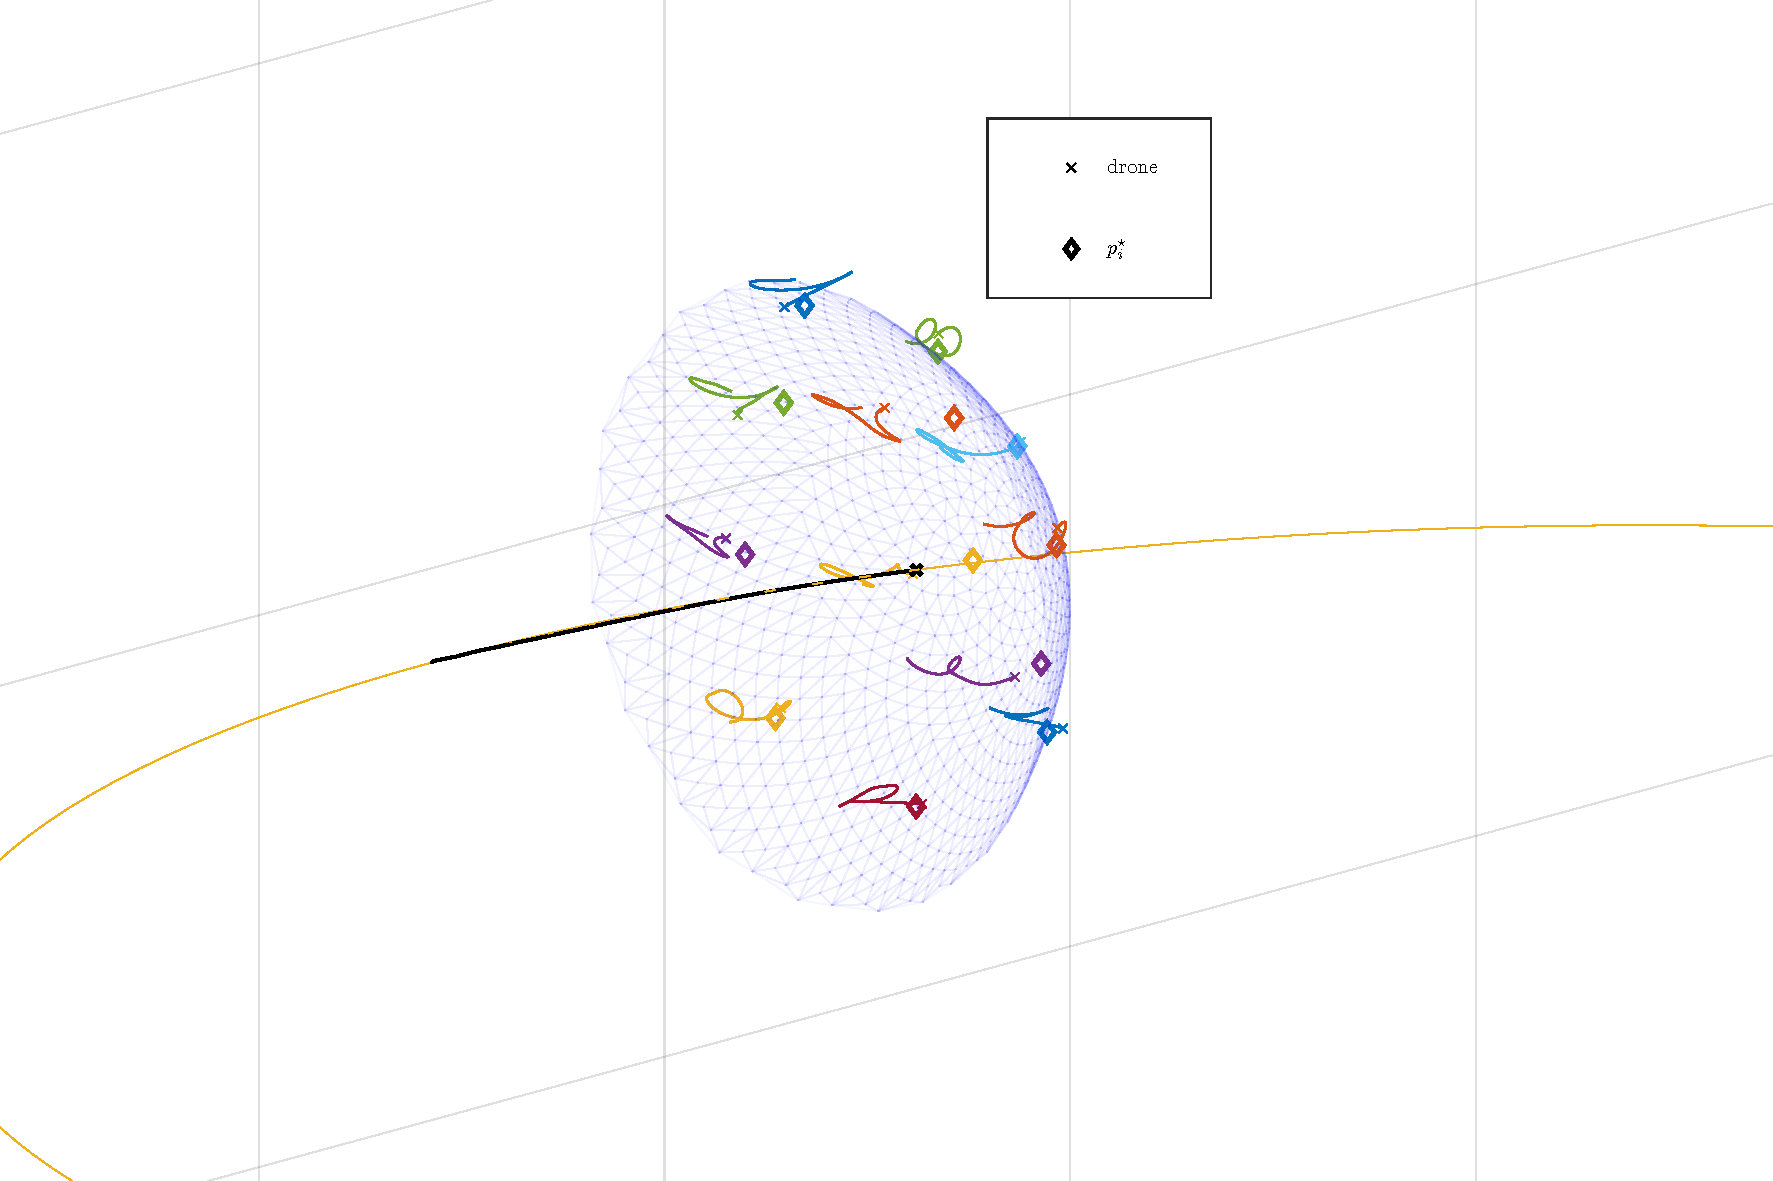
\includegraphics[width=6cm]{5-Figures/Chapter6/Simulation/decentralized_dijktra_t_3_close.pdf}
\end{minipage}

\vspace{0.3cm}

\begin{minipage}{0.12\textwidth}
t = 6:
\end{minipage}%
\begin{minipage}{0.85\textwidth}
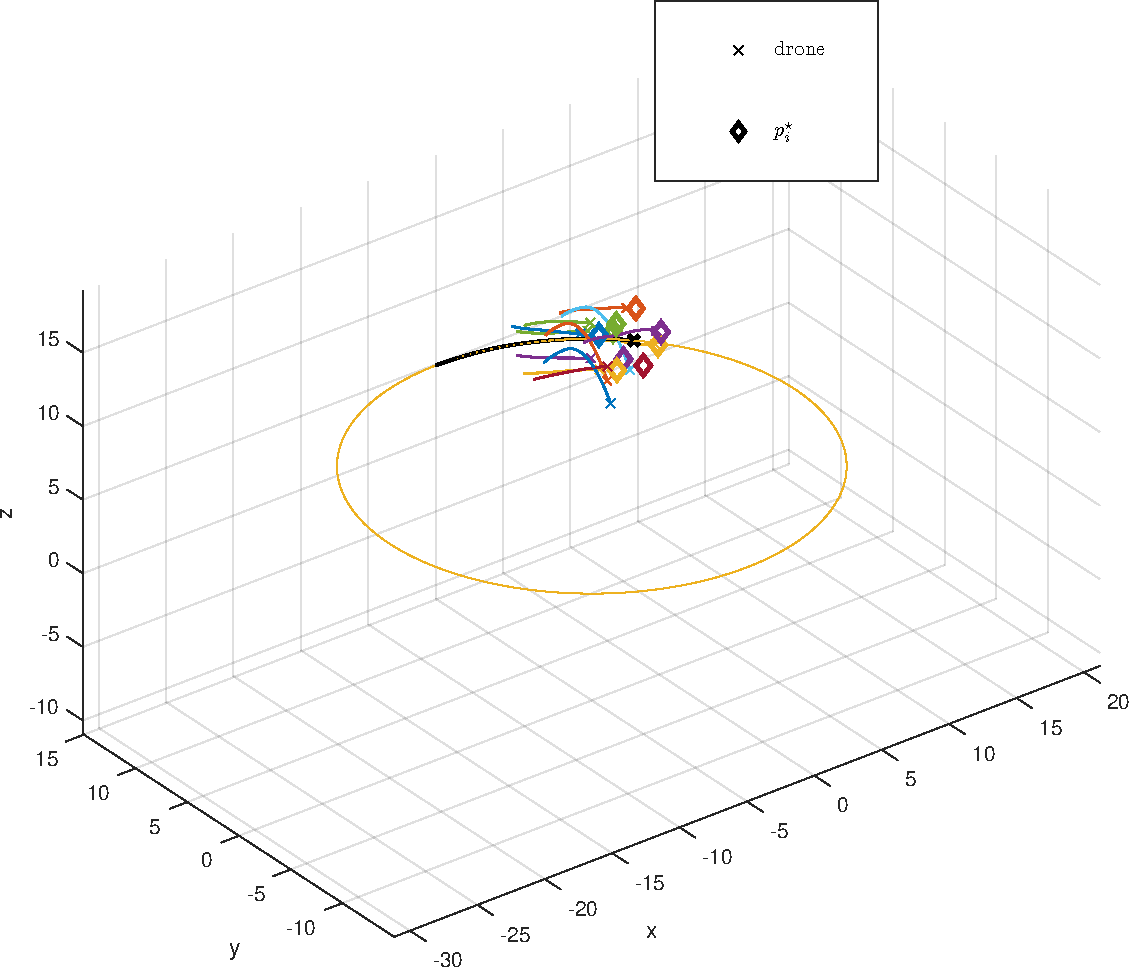
\includegraphics[width=6cm]{5-Figures/Chapter6/Simulation/decentralized_dijktra_t_6.pdf}\hfil   
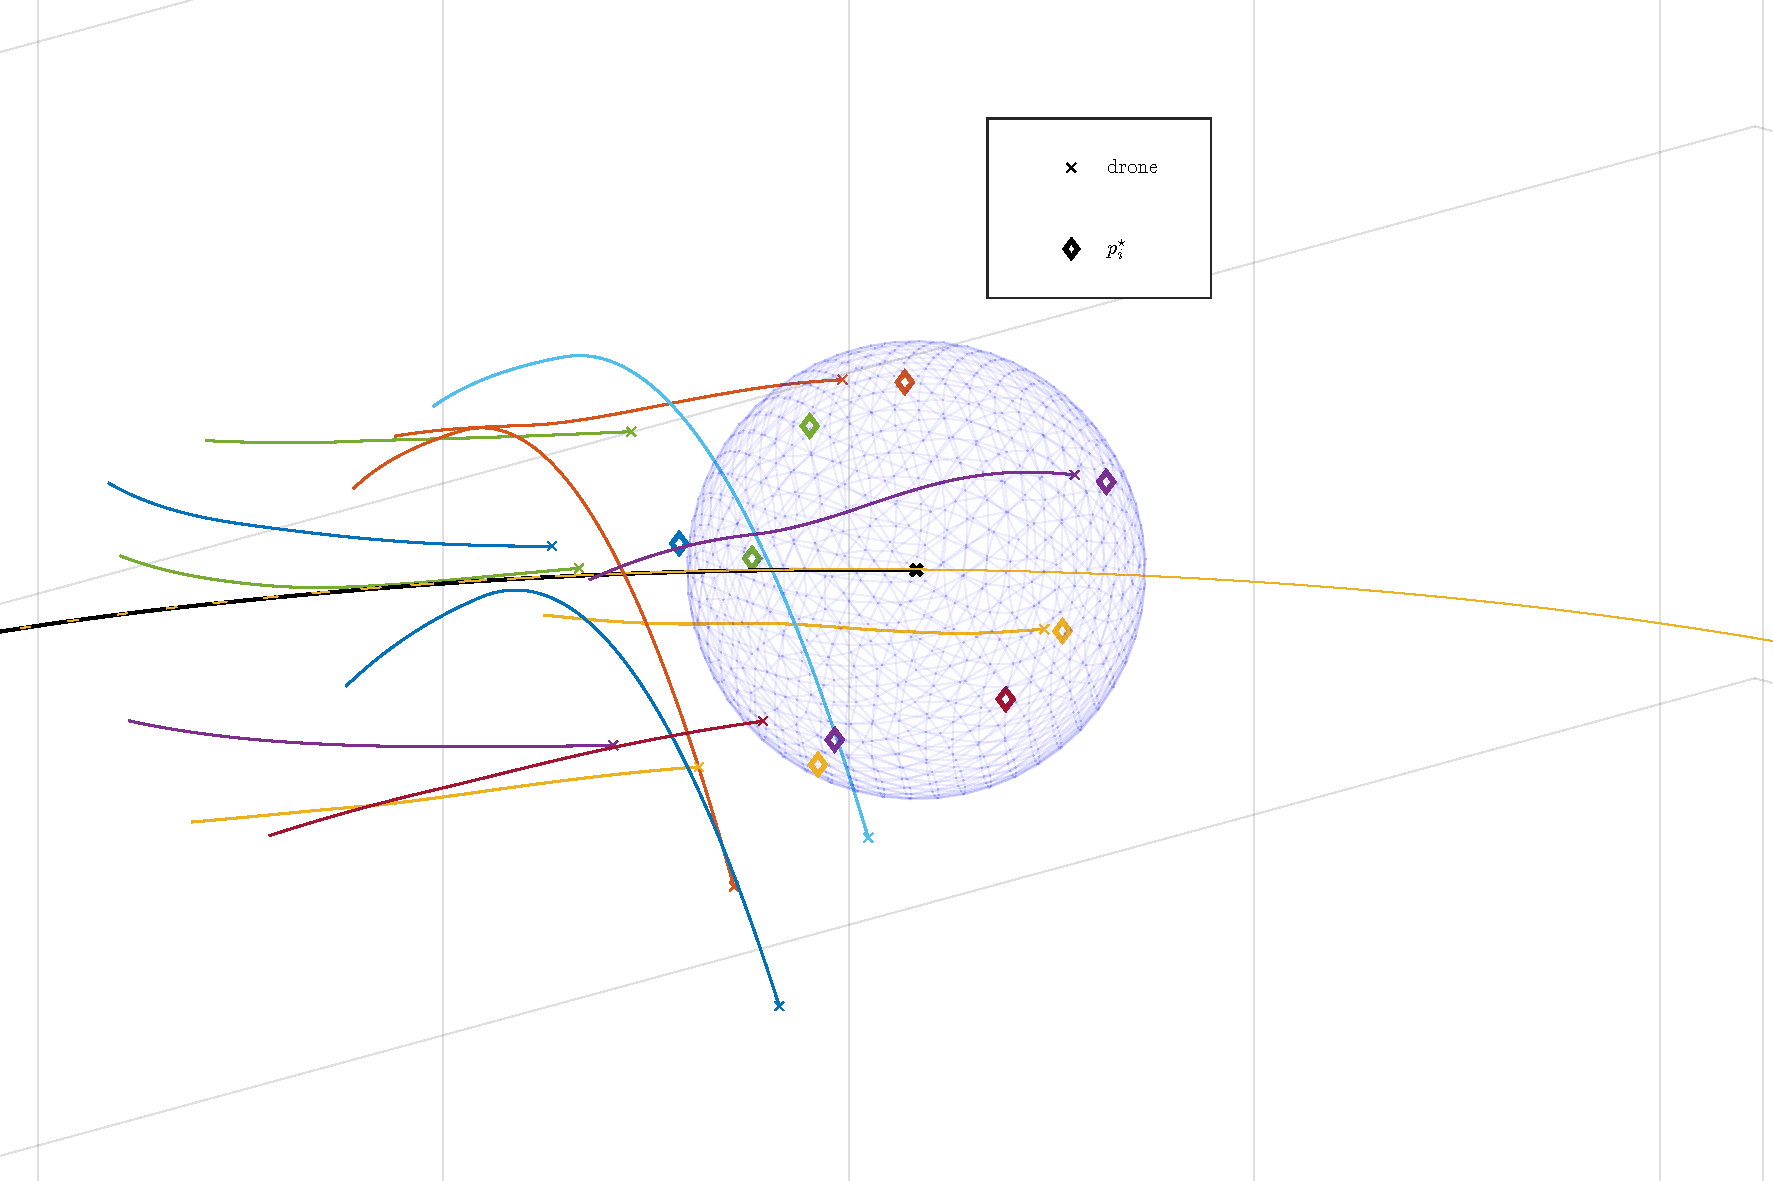
\includegraphics[width=6cm]{5-Figures/Chapter6/Simulation/decentralized_dijktra_t_6_close.pdf}
\end{minipage}

\vspace{0.3cm}
\begin{minipage}{0.12\textwidth}
t = 30:
\end{minipage}%
\begin{minipage}{0.85\textwidth}
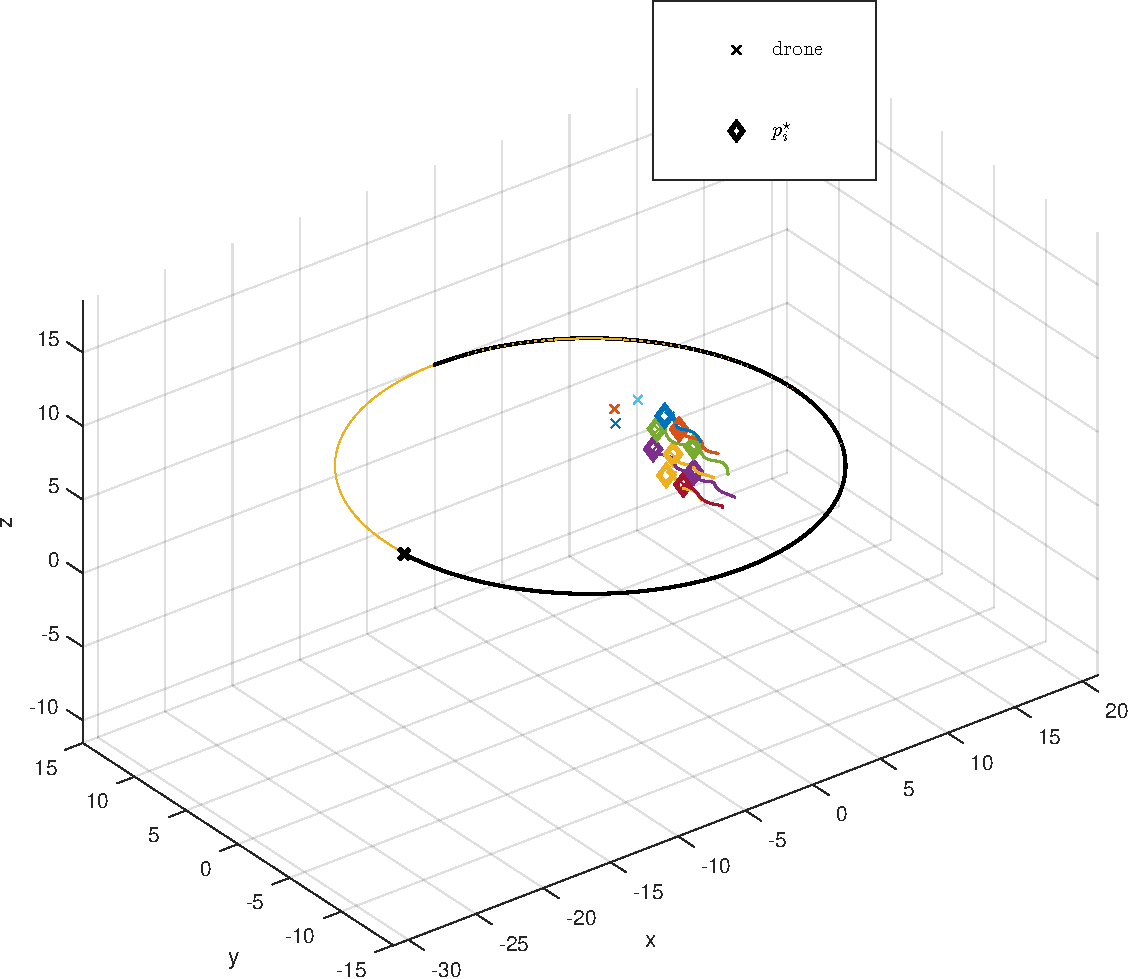
\includegraphics[width=6cm]{5-Figures/Chapter6/Simulation/decentralized_dijktra_t_30.pdf}\hfil   
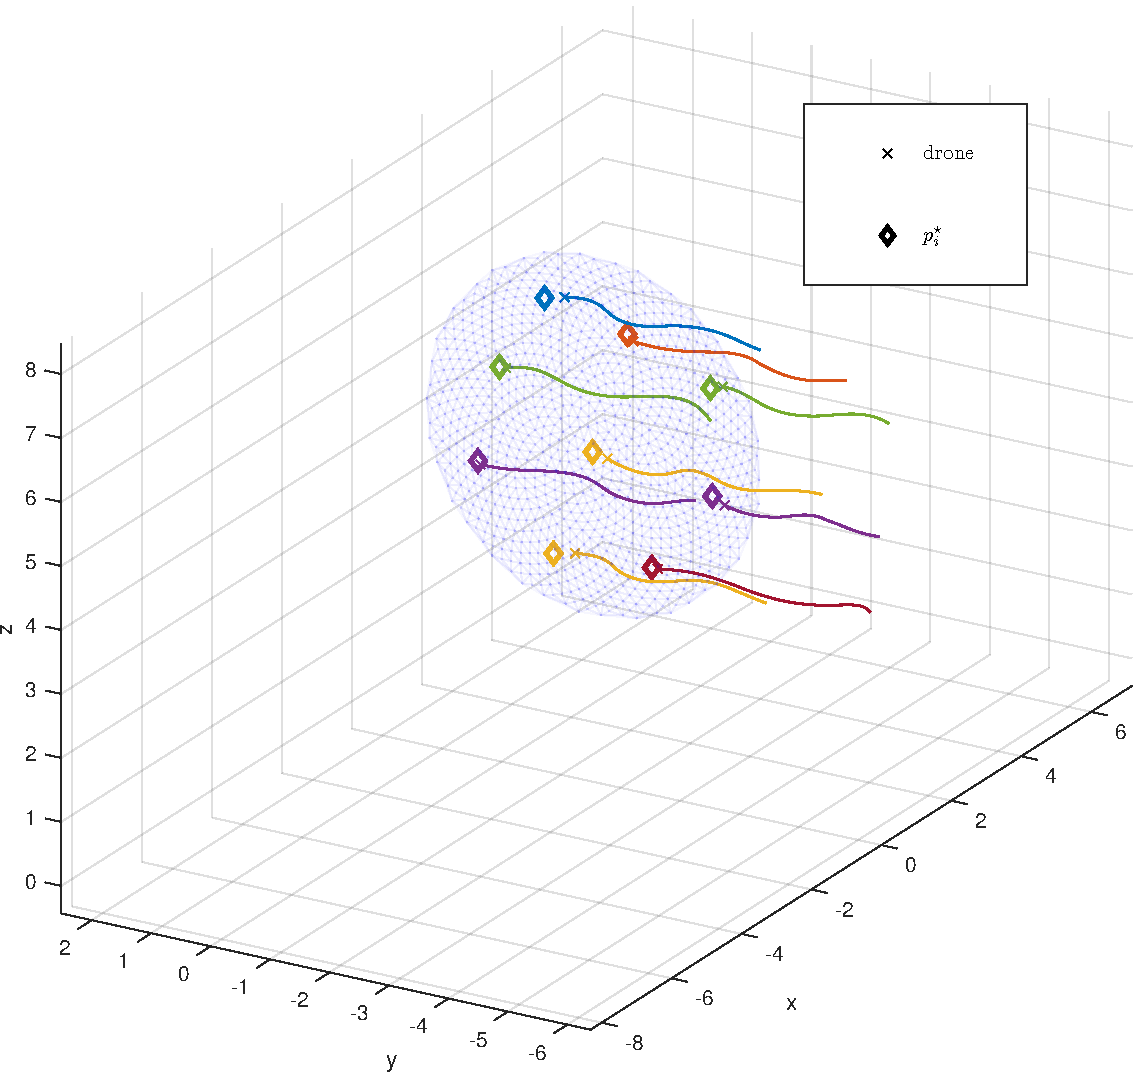
\includegraphics[width=6cm]{5-Figures/Chapter6/Simulation/decentralized_dijktra_t_30_close.pdf}
\end{minipage}
\caption{Simulation results through time}
\label{fig.6:simulation_results}
\end{figure}
